\chapter{Bonding in Transition Metal Complexes}

\section{Introduction}
The goal in this chapter is to put the study of transition metals on
the same theoretical footing as the other systems in covered in
the course. Transition metals are typically described using an
oxidation state formalism: this formalism allows crude predictions
about which states are allowed for which metals (e.g. Pd can form 0,
2, and 4 oxidation states, but not 3), but obscures finer details
about energetics and geometries of these compounds. We will see that
valence bond concepts, starting from the most stable configuration of
the fragments to understand what bonding can occur, can provide the
same predictive power in transition metals as it does for other parts
of the periodic table.

\section{Case Study: The Difference Between Pd and Pt Compounds}
We will motivate our discussion of transition metal chemistry by
contrasting the difference in chemical reactivity between Pd and Pt
compounds. Figure \ref{chaptm-fig-pdpt-rxns} shows the reductive
elimination of methane and ethane from Pd and Pt compounds. In the Pt
compounds, reductive elimination of ethane is not observed, but
reductive elimination of methane is fast. In contrast, with Pd
compounds redutive elimination of ethane is fast, and reductive
elimination of methane is so rapid that the starting compounds in
\ref{chaptm-fig-pdpt-rxns}(d) is so fast that the reactant is never
observed.

\begin{figure}
\begin{center}
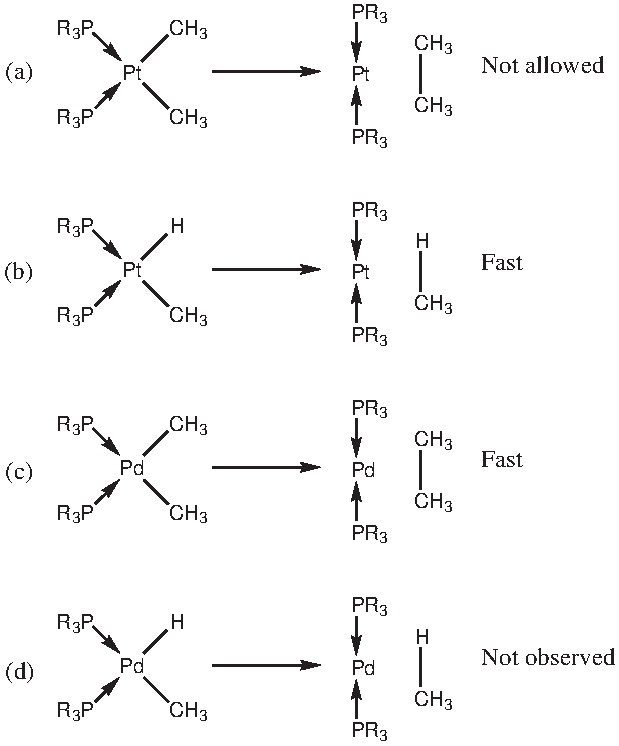
\includegraphics{chaptm-pdpt-rxns}
\end{center}
\caption{Comparison of reductive elimination chemistry of Pt and Pd
  compounds. (a) Elimimation of ethane from \chem{Pt^{II}} compounds
  is forbidden, but (b) elimination of methane is fast. In contrast,
  (c) elimination of ethane is fast from \chem{Pd^{II}} compounds, but
  (d) elimination of methane is so fast that the reactant is not
  observed.} 
\label{chaptm-fig-pdpt-rxns}
\end{figure}

Traditional inorganic chemistry, which considers the different
oxidation states that each metal can form, does not help us in
understanding this chemistry. All four reactions involve a transition
from a \chem{M^{II}} to a \chem{M^{0}}. To understand why these
different reactions occur as they do we must consider the nature of
the chemical bonds between the metal atoms and the relevant \chem{H}
and \chem{CH_3} fragments.

We begin by considering the relevant states of the metal atoms. Table
\ref{chaptm-tab-nipdpt} shows the relative energetics of the $s^1d^9$,
$s^2d^8$ and $d^{10}$ configurations of Ni, Pd, and Pt. We see that Pd
and Pt have different ground states: the ground state of Pd is the
$d^{10}$ state, with the $s^1d^9$ state 21.9 kcal/mol higher, and the
ground state of Pt is the $s^1d^9$ state, with the $d^{10}$ state 11.0
kcal/mol higher.

\begin{table}
\caption{Relative energies (in kcal/mol) of the $s^1d^9$,
$s^2d^8$ and $d^{10}$ configurations of Ni, Pd, and Pt.}
\label{chaptm-tab-nipdpt}
\begin{tabular}{ccccccc}\\ \hline
&\multicolumn{2}{c}{$s^1d^9$}&\multicolumn{2}{c}{$d^{10}$}&
 \multicolumn{2}{c}{$s^2d^8$}\\
& Exp. & DFT & Exp. & DFT & Exp. & DFT \\
Ni & 0.0 & 0.0 & 40.0 & 63.4 & 0.7 &  11.8\\
Pd & 0.0 & 0.0 & -21.9 & -2.05 & 56.0 & 61.6\\
Pt & 0.0 & 0.0 & 11.0 & 26.2 & 14.7 & 5.2 \\
\hline
\end{tabular}
\end{table}

Now we look at the chemical bonding typically seen in one of the
four-coordinate reactant states in Figure
\ref{chaptm-fig-pdpt-rxns}. A contour plot of the bonding orbital in
the \chem{(PR_3)_2Pt(CH_3)_2} compound is shown in Figure
\ref{chaptm-fig-ptch3ch3-contour}.  Here we see \emph{covalent}
bonding between the C $sp^3$ orbital and the Pt $s\pm d_{yz}$
orbital. This means that the oxidation state model that assumes that
two \chem{CH_3^-} ions bind to a \chem{(PR_3)_2Pt^{2+}} compound is
incorrect: the electrons in the bonding orbital are shared between the
Pt and C centers, and are not oxidized onto the C atom. 

\begin{figure}
\begin{center}
% need to make contour plot of ptch3ch3 bonding orbital
\end{center}
\caption{Contour plot of the bonding orbital in the 
\chem{(PR_3)_2Pt(CH_3)_2} compound that shows covalent bonding between
the C $sp^3$ orbital and the Pt $s\pm d_{yz}$ orbital.}
\label{chaptm-fig-ptch3ch3-contour}
\end{figure}

Because the Pt-C bond is covalent, it means that we must have two
half filled orbitals on the metal atom to bond to the two \chem{CH_3}
radical orbitals. The $d^{10}$ configuration doesn't have any partially
filled orbitals, which means that to form the \chem{(PR_3)_2M(CH_3)_2}
complexes, the metal atom must be in the $s^1d^9$ state.
The half-filled $3s$ and $3d_{x^2-y^2}$ hybridize to form two $s-d$ lobe
orbitals, pointing in the $x$ and the $y$ directions, as shown in
Figure \ref{chaptm-sd-hybr}.

\begin{figure}
\begin{center}
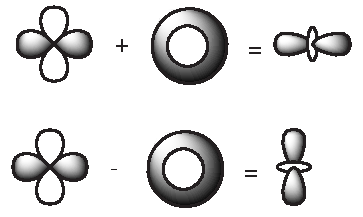
\includegraphics{chaptm-sd-hybr}
\end{center}
\caption{Linear combinations of the $3d_{x^2-y^2}$ and $3s$ orbitals
  form $s-d$ lobe orbitals pointing in the $x$ and $y$ directions.}
\label{chaptm-sd-hybr}
\end{figure}

In contrast, the bonding between the \chem{PR_3} groups in the
\chem{(PR_3)_2M} compounds is \emph{dative}: the lone pair orbital on
the P atom donates into an empty orbital on the metal atom. There are
low-lying empty orbitals in the metal $d^{10}$ configuration, but
there are none in the metal $s^1d^9$ configuration. Which means to
form the \chem{(PR_3)_2M} species on the right of Figure
\ref{chaptm-fig-pdpt-rxns} we need a $d^{10}$ configuration.

Thus, the reductive elimination process shown in Figure
\ref{chaptm-fig-pdpt-rxns} involves the metal atom going from a
$s^1d^9$ configuration to a $d^{10}$ configuration. Because in Pd the
$d^{10}$ configuration is more stable by 21.9 kcal/mol than the
$s^1d^9$ configuration, whereas in Pt the $d^{10}$ configuration is
less stable by 11.0 kcal/mol than the $s^1d^9$, we would expect
reductive elimination process to be more favorable in Pd than it is in
Pt---the general trend seen in the reactions in Figure
\ref{chaptm-fig-pdpt-rxns}!

\begin{figure}
\begin{center}
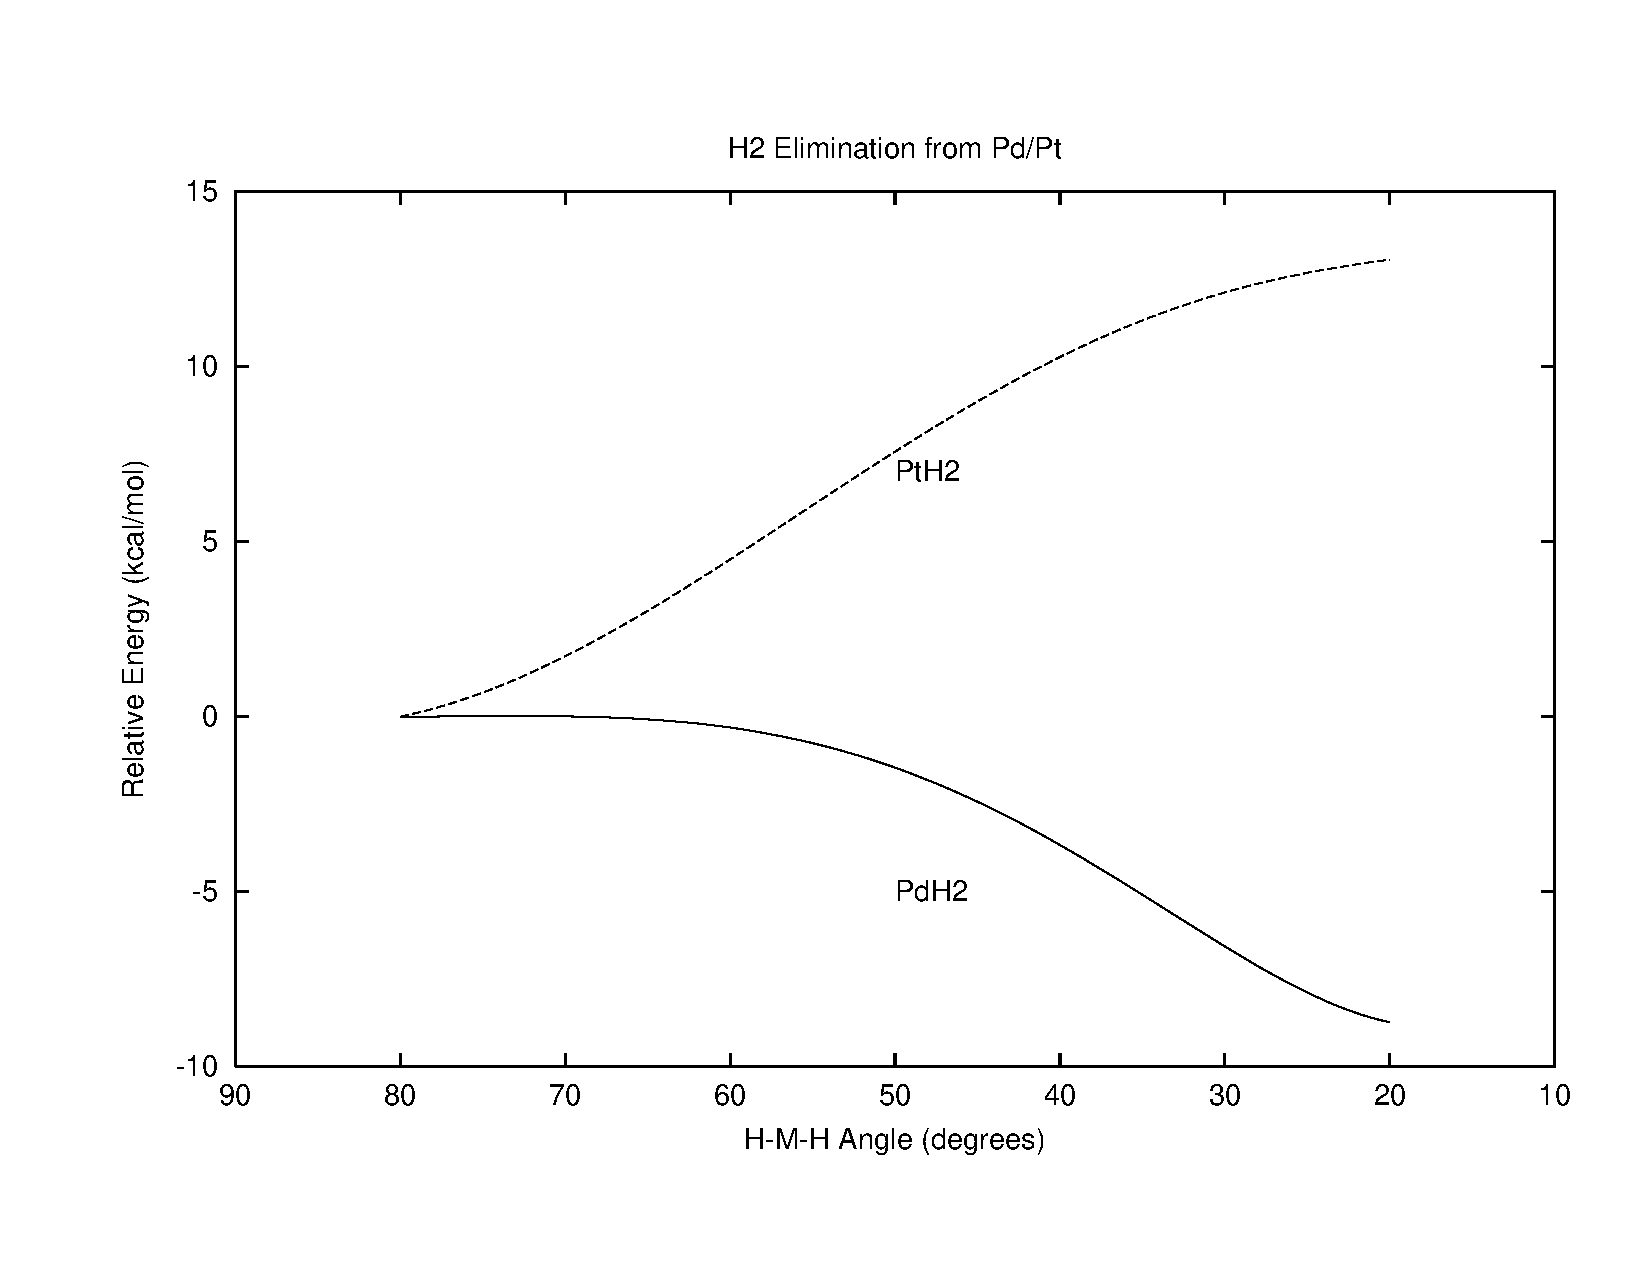
\includegraphics[scale=0.5,angle=-90]{chaptm-fig-h2}
\end{center}
\caption{Comparison of \chem{H_2} elimination reactions from Pd and
  Pt. Note that the final difference in energy is on the same order as
  the 20--30 kcal/mol predicted by the differences in the
  $s^1d^9-d^{10}$ excitation energies from Table
  \ref{chaptm-tab-nipdpt}.}
\label{chaptm-fig-h2}
\end{figure}

\begin{figure}
\begin{center}
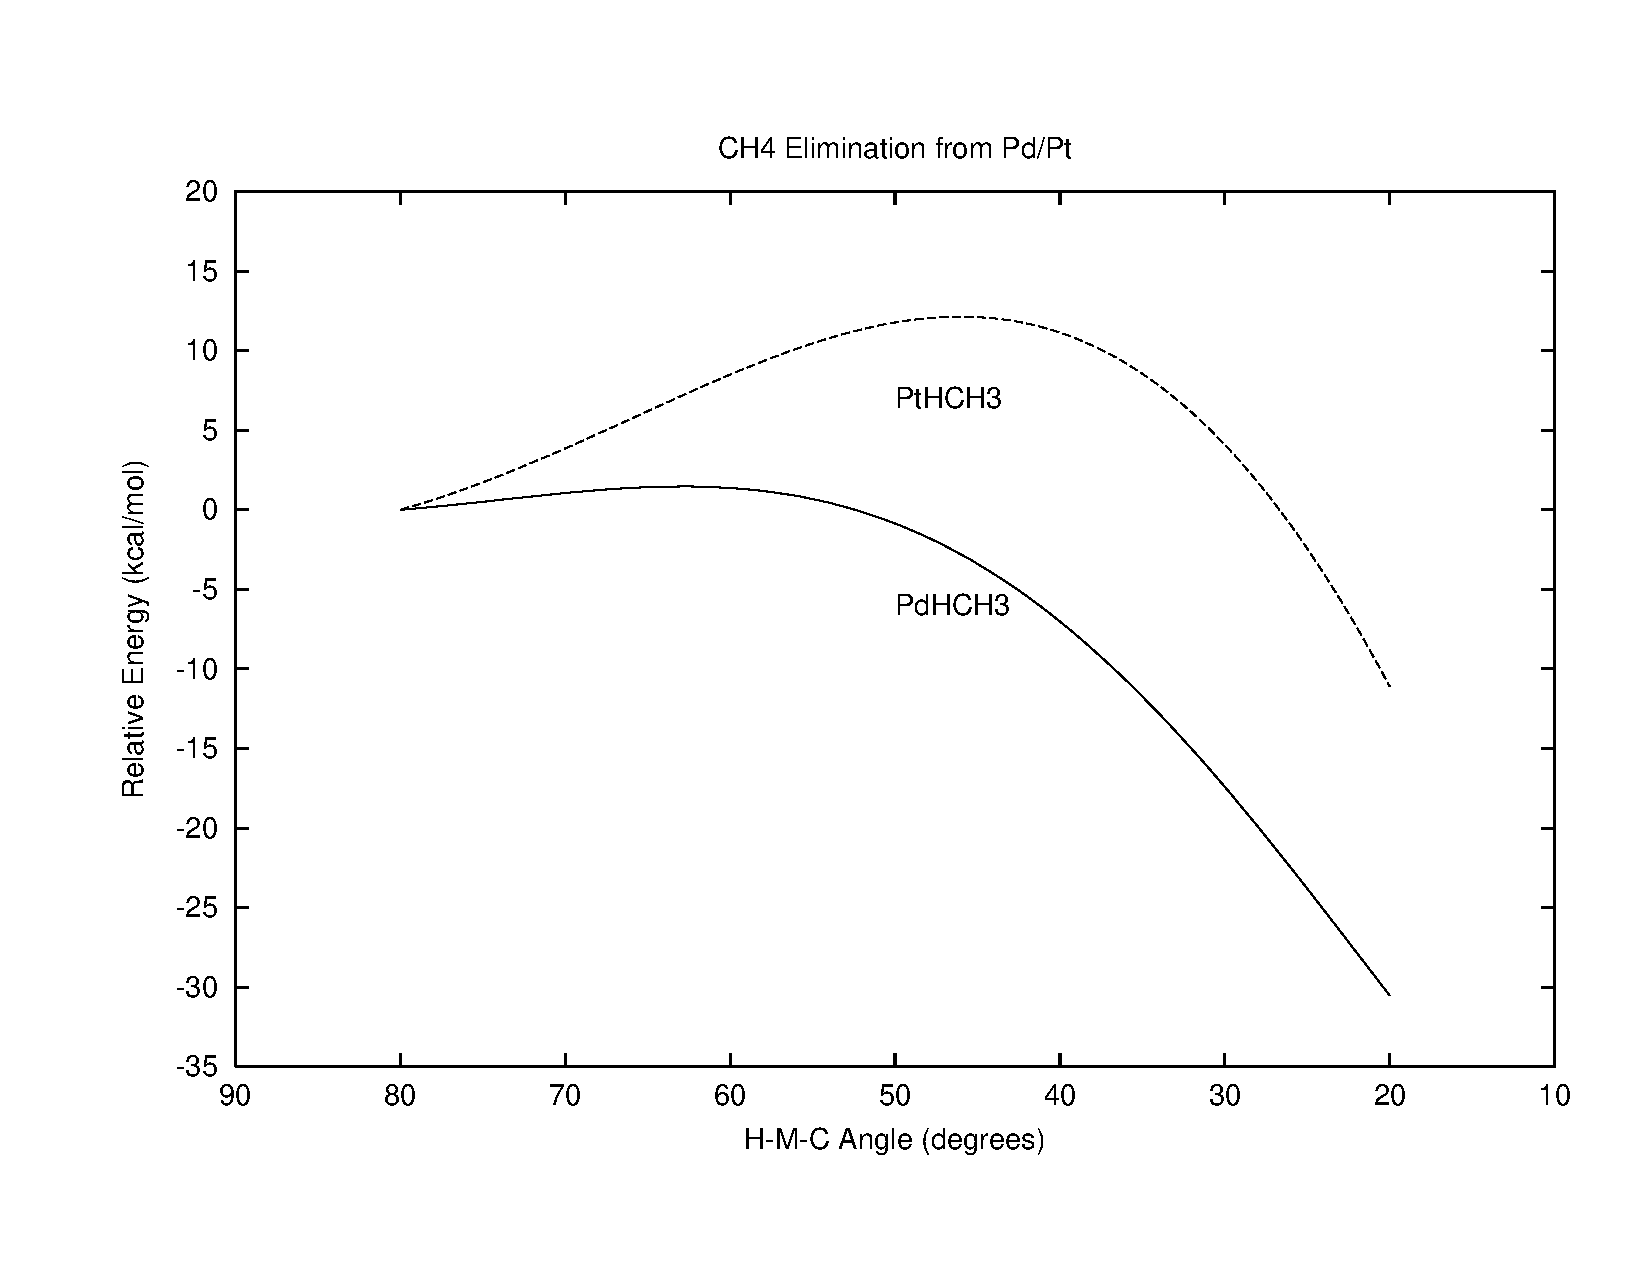
\includegraphics[scale=0.5,angle=-90]{chaptm-fig-hch3}
\end{center}
\caption{Comparison of \chem{CH_4} elimination reactions from Pd and
  Pt. Note that the final difference in energy is on the same order as
  the 20--30 kcal/mol predicted by the differences in the
  $s^1d^9-d^{10}$ excitation energies from Table
  \ref{chaptm-tab-nipdpt}. In contrast to Figure \ref{chaptm-fig-h2},
  here we see that both reactions have a slight barrier, arising from
  the fact that \chem{CH_3} forms more directed bonds than does
  \chem{H}, destabilizing the transition state.}
\label{chaptm-fig-hch3}
\end{figure}

Results from the elimination of \chem{H_2} and \chem{CH_4} from Pd and
Pt are shown in Figures \ref{chaptm-fig-h2} and
\ref{chaptm-fig-hch3}. In both cases, the final difference between the
two states is roughly the same as we would expect from the differences
in the $s^1d^9-d^{10}$ excitation energies from Table
\ref{chaptm-tab-nipdpt}. However, the elimination of \chem{CH_4} has a
barrier, arising from the fact that \chem{CH_3} forms a directed bond
with a C $sp$ lobe orbital, which can bond with either the reactant or
the product state, but not both. In contrast, the $s$ orbital in
\chem{H} is spherical, and it can bond to both the reactant and the
product simultaneously. The result of this difference is that when
\chem{H_2} is eliminated from \chem{(PH_3)_2PdH_2} is has no barrier,
but when \chem{CH_4} is eliminated from \chem{(PH_3)_2PdHCH_3} there
is a small barrier. When \chem{C_2H_6} is eliminated from
\chem{(PH_3)_2Pd(CH_3)_2} there is an even higher barrier.

The previous discussion motivates us to look more quantitatively into
transition metal bonding, which we will attempt in the following
sections. 

\section{Valence Bonds to Transition Metals}
The previous section showed an example of how knowledge of the
different electronic states of transition metal atoms can help explain
the difference between reductive elimination chemistry exhibited by Pd
and Pt. This section will delve deeper into these concepts.

\subsection{VB vs Oxidation State Concepts}
\label{vb-tm-sect}
Traditionally the bonding of transition metals to different moities is
explained using oxidation states.
\begin{enumerate}
\item A \chem{M-H} bond is assumed to
  involve ionic bonding between a \chem{M^+} and \chem{H^-};
\item A \chem{M=O} is assumed to be ionic between \chem{M^{2+}} and
\chem{O^{2-}};
\item A \chem{M=CH_2} is assumed to be ionic between \chem{M^{2+}} and
\chem{CH_2^{2-}};
\end{enumerate}
and so on. However, in assuming that the metal electron is completely
ionized, we lose a lot of structural and energetic information about
the bonding in these compounds. It turns out that the bonds to
transition metals can be quite covalent, and that by using simple VB
concepts we can gain real predictive power regarding the nature of
these compounds.

\begin{figure}
\begin{center}
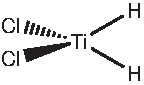
\includegraphics{chaptm-cl2tih2}
\end{center}
\caption{\chem{Cl_2TiH_2}.}
\label{chaptm-cl2tih2}
\end{figure}

Consider the bonding in \chem{Cl_2TiH_2} (Figure
\ref{chaptm-cl2tih2}). If we examine the \chem{Ti-Cl} bonds, we see
that in this case, the oxidation state formatlism is mostly correct,
and that the bonds look like two \chem{Cl^-} atoms bonded to a
\chem{Ti^{2+}} atom, because Cl atoms are much more electronegative
than a Ti atom, and completely ionize the electron. The ground state
of Ti is $(4s)^2(3d)^2$, so the Cl can ionize either a $4s$ or a $3d$
electron. Of the two, the $4s$ electron is easier to ionize, both
because the $4s$ shell is farther away from then atom than the $3d$
shell, and because the $d-d$ exchange integrals give the $d$ electrons
extra stability.

The \chem{Ti-H} bonds, however, are qualitatively different from the
\chem{Ti-Cl} bonds; these are much more covalent. Since we have
already ionized the $4s$ electrons, all that is left is two $3d$
electrons. We would like to form two good $\sigma$ bonds with these
orbitals.

For $d$ orbitals, the lobe-like $d_{z^2}$ orbitals (which actually
have the Cartesian components $2z^2-x^2-y^2 = 3z^2-R^2$) make much
better bonds than the $d_{xy}$ or $d_{x^2-y^2}$  orbitals because the
$z^2$ orbitals have their electron density more concentrated along
a single bonding direction, and can thus form better overlap with
other orbitals. We know we can make a single $z^2$ orbital, can we
make a second one? It turns out that we can. We can make a linear
combination of the remaining $d$ orbitals that forms an identical lobe
to the $d_{z^2}$ orbital, but rotated $54.7^\circ$. This means that
$\sigma$ bonds to $d$ orbitals will have a natural angle of either
$54.7^\circ$ or $180-54.7=125.3^\circ$ (see Figure
\ref{chaptm-two-z2-lobes}). 

\begin{figure}
\begin{center}
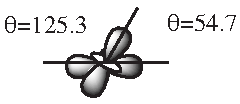
\includegraphics{chaptm-two-z2-lobes}
\end{center}
\caption{We can take linear combinations of the $d$ orbitals to form
  two $d_{z^2}$-like orbitals that have an angle of $54.7^\circ$
  between them.}
\label{chaptm-two-z2-lobes}
\end{figure}

Thus, there are two different classes of bonding in
\chem{Cl_2TiH_2}. The \chem{Ti-Cl} bonds are \emph{ionic}: the Cl
ionizes the electron out of the $4s$ orbitals. The \chem{Ti-H} bonds
are \emph{covalent}: the remaining $3d$ orbitals hybridize to form two
lobe orbitals that can form covalent bonds. We will sometimes draw the
bonds as in Figure \ref{chaptm-cl2tih2_arrows} to emphasize this
distinction.

\begin{figure}
\begin{center}
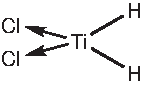
\includegraphics{chaptm-cl2tih2_arrows}
\end{center}
\caption{The bonding in \chem{Cl_2TiH_2}, with arrows emphasizing the
  distinction between the ionic \chem{Ti-Cl} bonds and the covalent
  \chem{Ti-H} bonds.}
\label{chaptm-cl2tih2_arrows}
\end{figure}

Our procedure for determining the bonding in transition metal
compounds is now as follows:
\begin{enumerate}
\item Start with the atomic configuration of the metal;
\item Consider bonds to the electronegative ligands, using electrons
  from the $4s$ orbitals, which are easier to ionize;
\item Now make bonds between the remaining orbitals and the less
  electronegative ligands.
\end{enumerate}
Consider the bonding in \chem{(Cp)_2Ti=CH_2}, Figure
\ref{chaptm-cp2tich2}. The \chem{Cp}---cyclopentadienyl---ligands are
very electronegative, because adding an additional electron makes them
aromatic. Thus, they act chemically very much like \chem{Cl} ligands,
forming symmetric bonds between the center of the ring with the metal
atom (organometallic chemists refer to this bonding where all five
ligand atoms are equivalent in their bonding to the metal as $\eta^5$
bonding). We assume that the \chem{Cp} rings will ionize the $4s$
electrons from the Ti atom. Now we are left with two $3d$ atoms to
bond to the \chem{CH_2}. We would like to form a $\sigma$ and a $\pi$
orbital to \chem{CH_2}, analogous to the bonding in ethylene. For this
type of bonding it turns out that forming two $d_{z^2}$ lobe orbitals
as in Figure \ref{chaptm-two-z2-lobes} is \emph{not} we desire, as the
second lobe forms a very poor $\pi$ bond. It turns out, however, that
a $d_{xz}$ orbital can make a very good $\pi$ bond with the C $p_x$
orbital, as shown in Figure \ref{chaptm-dpi}.

\begin{figure}
\begin{center}
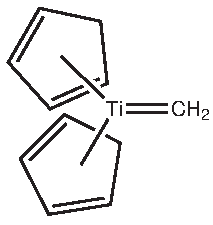
\includegraphics{chaptm-cp2tich2}
\end{center}
\caption{\chem{(Cp)_2Ti=CH_2}}
\label{chaptm-cp2tich2}
\end{figure}

\begin{figure}
\begin{center}
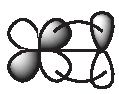
\includegraphics{chaptm-dpi}
\end{center}
\caption{$\pi$ bonding between a $d_xz$ orbital on Ti and a $p_x$
  orbital on C; it is assumed that the $\sigma$ bonding is in the $z$
  direction here.}
\label{chaptm-dpi}
\end{figure}


\subsection{Transition Metal Hydrides}
[Cite Ohanessian/Goddard ACR for this entire section...] We now turn
our attention to how the valence bond concepts may be used in a
systematic way to understand how transition metal cations bond to
hydrogen atoms. We begin with a consideration of the ground states of
the transition metal cations. The ground state of \chem{M^+} is
typically either $d^n$ or $s^1d^{n-1}$, where $n$ is the number of
valence electrons. The exceptions to this rule are \chem{Y^+} and
\chem{Hf^+}, which are both $s^2d^{n-2}$ configurations. Figure
\ref{chaptm-esplit} shows the energy difference between the $d^n$ and
$s^1d^{n-1}$ states for the transition metals.

\begin{figure}
\begin{center}
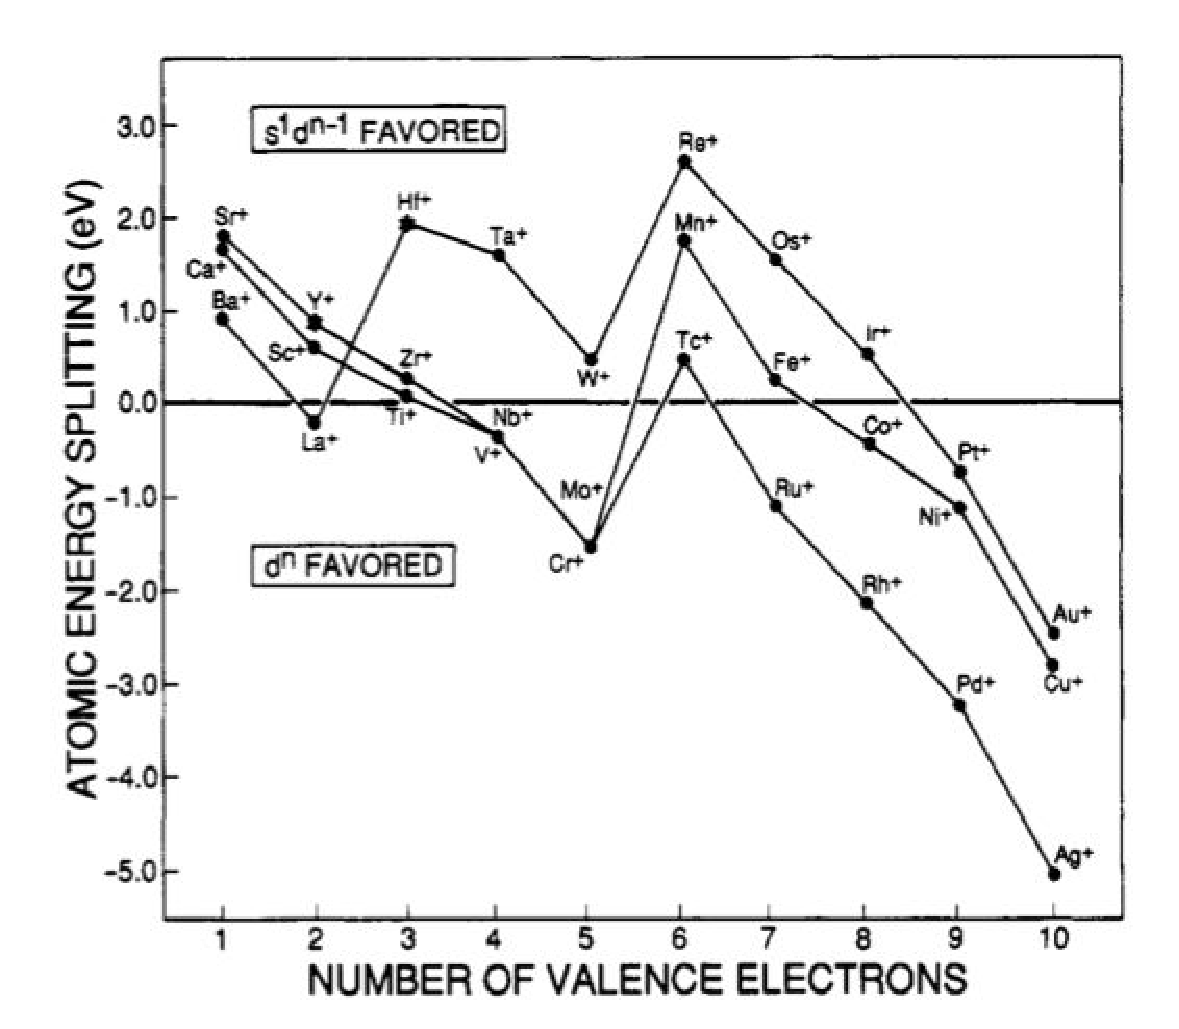
\includegraphics[scale=0.5]{chaptm-esplit}
\end{center}
\caption{Energy difference between the lowest metal cation electronic
states arising from $d^n$ and $s^1d^{n-1}$ configurations: $\Delta E =
E_{d^n} - E_{s^1d^{n-1}}$. In each case the experimental states have
been averaged over $J$ to obtain $LS$ state energies. The stars on
\chem{Y^+} and \chem{Hf^+} indicate that $s^2d^{n-2}$ is the ground
configuration in these cases.}
\label{chaptm-esplit}
\end{figure}

\begin{table}
\label{tmh-first}
\caption{Calculated ground state symmetries, bond lengths, and bond
energies of first row transition metal hydride cations. The
parentheses after each state contain the total number of electrons in
the nonbonding orbitals of different symmetries.}
\begin{tabular}{cccc}\hline 
Species  & State & $R_{MH}$ \AA& $D_0$ (kcal/mol) \\ \hline
\chem{CaH^+} & $^1\Sigma^+ (\sigma^0\pi^0\delta^0)$ & 1.940 & 44.7 \\
\chem{ScH^+} & $^2\Delta (\sigma^0\pi^0\delta^1)$   & 1.810 & 55.2 \\
\chem{TiH^+} & $^3\Phi (\sigma^0\pi^1\delta^1)$     & 1.730 & 54.0 \\
\chem{VH^+}  & $^4\Delta (\sigma^0\pi^2\delta^1)$   & 1.662 & 43.6 \\
\chem{CrH^+} & $^5\Sigma^+ (\sigma^0\pi^2\delta^2)$ & 1.602& 24.3\\
\chem{MnH^+} & $^6\Sigma^+ (\sigma^1\pi^2\delta^2)$ & 1.702& 39.6\\
\chem{FeH^+} & $^5\Delta (\sigma^1\pi^2\delta^3)$   & 1.653& 47.0\\
\chem{CoH^+} & $^4\Phi (\sigma^1\pi^3\delta^3)$     & 1.606& 43.6\\
\chem{NiH^+} & $^3\Delta (\sigma^1\pi^4\delta^3)$   & 1.561& 35.7\\
\chem{CuH^+} & $^2\Sigma^+ (\sigma^1\pi^4\delta^4)$ & 1.513& 20.9\\
\chem{ZnH^+} & $^1\Sigma^+ (\sigma^2\pi^4\delta^4)$ & 1.545& 52.4\\
\\ \hline
\end{tabular}
\end{table}

\begin{table}
\label{tmh-second}
\caption{Calculated ground state symmetries, bond lengths, and bond
energies of second row transition metal hydride cations. The
parentheses after each state contain the total number of electrons in
the nonbonding orbitals of different symmetries.}
\begin{tabular}{cccc}\hline
Species  & State & $R_{MH}$ \AA& $D_0$ (kcal/mol) \\ \hline
\chem{SrH^+} & $^1\Sigma^+ (\sigma^0\pi^0\delta^0)$ & 2.079 & 44.1 \\
\chem{YH^+} & $^2\Sigma^+ (\sigma^1\pi^0\delta^0)$  & 1.892 & 57.8 \\
\chem{ZrH^+} & $^3\Phi (\sigma^0\pi^1\delta^1)$     & 1.857 & 54.6 \\
\chem{NbH^+} & $^4\Delta (\sigma^0\pi^2\delta^1)$   & 1.764 & 48.7 \\
\chem{MoH^+} & $^5\Sigma^+ (\sigma^0\pi^2\delta^2)$ & 1.708 & 31.2 \\
\chem{TcH^+} & $^6\Sigma^+ (\sigma^1\pi^2\delta^2)$ & 1.719 & 46.3 \\
\chem{RuH^+} & $^3\Sigma^- (\sigma^0\pi^4\delta^2)$ & 1.581 & 31.7 \\
\chem{RhH^+} & $^2\Delta (\sigma^0\pi^4\delta^3)$   & 1.539 & 34.8 \\
\chem{PdH^+} & $^1\Sigma^+ (\sigma^0\pi^4\delta^4)$ & 1.512 & 40.6 \\
\chem{AgH^+} & $^2\Sigma^+ (\sigma^1\pi^4\delta^4)$ & 2.428 & 2.1 \\
\chem{CdH^+} & $^1\Sigma^+ (\sigma^2\pi^4\delta^4)$ & 1.709 & 42.0 \\
\\ \hline
\end{tabular}
\end{table}

\begin{table}
\label{tmh-third}
\caption{Calculated ground state symmetries, bond lengths, and bond
energies of third row transition metal hydride cations. The
parentheses after each state contain the total number of electrons in
the nonbonding orbitals of different symmetries.}
\begin{tabular}{cccc}\hline
Species  & State & $R_{MH}$ \AA& $D_0$ (kcal/mol) \\ \hline
\chem{BaH^+} & $^1\Sigma^+ (\sigma^0\pi^0\delta^0)$ & 2.202 & 50.9 \\
\chem{LaH^+} & $^2\Delta (\sigma^0\pi^0\delta^1)$   & 2.093 & 60.4 \\
\chem{HfH^+} & $^3\Delta (\sigma^1\pi^0\delta^1)$   & 1.786 & 54.9 \\
\chem{TaH^+} & $^4\Sigma^- (\sigma^1\pi^2\delta^0)$ & 1.741 & 54.0 \\
\chem{WH^+}  & $^5\Pi (\sigma^1\pi^1\delta^2)$      & 1.701 & 49.9 \\
\chem{ReH^+} & $^6\Sigma^+ (\sigma^1\pi^2\delta^2)$ & 1.659 & 44.5 \\
\chem{OsH^+} & $^5\Pi (\sigma^1\pi^3\delta^2)$      & 1.605 & 56.2 \\
\chem{IrH^+} & $^4\Sigma^- (\sigma^1\pi^4\delta^2)$ & 1.560 & 65.8 \\
\chem{PtH^+} & $^1\Sigma^+ (\sigma^0\pi^4\delta^4)$ & 1.519 & 62.9 \\
\chem{AuH^+} & $^2\Sigma^+ (\sigma^1\pi^4\delta^4)$ & 1.539 & 33.4 \\
\chem{HgH^+} & $^1\Sigma^+ (\sigma^2\pi^4\delta^4)$ & 1.627 & 48.6 \\
\\ \hline
\end{tabular}
\end{table}

We now will use the valence bond rules that we outlined in section
\ref{vb-tm-sect} to guide us in the construction of the \chem{M^+-H}
bond. 

\begin{enumerate}
\item We start with ground state of the \chem{M^+} species, either the
$d^n$ or the $s^1d^{n-1}$ configuration, as shown in figure
\ref{chaptm-esplit}. 
\item We then redistribute the electrons so as to
reserve a singly occupied $\sigma$ orbital to bond to the H $1s$
electron, keeping the total number of unpaired orbitals fixed, and
minimizing the number of nonbonding $\sigma$ electrons that might
destabilize the bonding orbital. Typically, early transition metal
hydrides avoid having nonbonding $\sigma$ orbitals altogether,
whereas late transition metal hydrides have one to minimize repulsions
with $\pi$ and $\delta$ nonbonding orbitals. 
\item Given a choice in the distribution of the remaining electrons
between $\pi$ and $\delta$ orbitals, we choose the one with the lowest
total electron repulsion in the atom.
\item In some cases, the electronic configuration of \chem{M^+} that
minimizes the nonbonding repulsion corresponds to an excited state of
the \chem{M^+} atom; when the promotion energy to this state is
sufficiently low, the ground state of \chem{MH^+} is formed with this
excited configuration.
\end{enumerate}

As an example of these rules, consider the bonding in
\chem{ScH^+}. Figure \ref{chaptm-esplit} indicates that the $s^1d^1$
state is the ground state. We reserve the electron in the $s$ orbital
to bond to the H $1s$ electron, and then determine whether the $d$
electron is $\sigma$, $\pi$, or $\delta$. $\sigma$ is the worst, since
is has to be orthogonal to the bonding orbital. The $\delta$ orbital
has the lowest interaction with the bonding electrons, which leads to
a $^2\Delta$ state for the species.

Tables \ref{tmh-first}--\ref{tmh-third} show the results for all three
rows of the periodic table.

% GO/WAG paper also has sections on hybridization, charge transfer,
% bond lengths, and bond energies, which I'm excluding from here.



\section{Polymerization Catalysis}
\subsection{Ziegler-Natta Catalysis}
\subsection{ROMP Catalysis}

%\section{Hemoglobin and Myoglobin}
%\section{The Spectator Oxo Effect}
